% ============================================================
% QRS 2026 — MACCP: Conformal Prediction Sets for Multi-Class
%                    Bug Triage via Cross-Model Agreement
% ============================================================
\documentclass[conference]{IEEEtran}

% ---- Packages ----
\usepackage{amsmath,amssymb}
\usepackage{booktabs}
\usepackage{graphicx}
\usepackage{multirow}
\usepackage{xcolor}
\usepackage{tikz}
\usetikzlibrary{arrows.meta,positioning,shapes.geometric,fit,calc}
\usepackage{algorithm}
\usepackage{algpseudocode}
\usepackage{url}
\usepackage{cite}
\usepackage{balance}
\usepackage{listings}
\usepackage{enumitem}

% ---- Compact lists ----
\setlist{nosep,leftmargin=*}

% ---- Math shortcuts ----
\newcommand{\calD}{\mathcal{D}}
\newcommand{\calC}{\mathcal{C}}
\newcommand{\indicator}[1]{\mathbb{1}\!\left[#1\right]}
\newcommand{\PP}{\mathbb{P}}
\DeclareMathOperator*{\argmax}{arg\,max}
\DeclareMathOperator{\Quantile}{Quantile}
\newcommand{\pp}{\text{pp}}

% ---- Listing style for explanation box ----
\lstdefinestyle{explbox}{
  basicstyle=\ttfamily\scriptsize,
  frame=single,
  framerule=0.4pt,
  xleftmargin=2pt,
  xrightmargin=2pt,
  breaklines=true,
  columns=fullflexible,
}

% ============================================================
\begin{document}

\title{Conformal Prediction Sets for Multi-Class Bug Triage:\\How Cross-Model Agreement Enables Reliable Automation}

\author{
\IEEEauthorblockN{[Author Names Redacted for Review]}
\IEEEauthorblockA{[Affiliations Redacted for Review]}
}

\maketitle

% ============================================================
% ABSTRACT
% ============================================================
\begin{abstract}
Machine learning classifiers for software bug triage produce point predictions without reliability guarantees, leaving practitioners unable to distinguish trustworthy assignments from unreliable ones. We apply conformal prediction---a distribution-free framework that produces prediction \emph{sets} with formal coverage guarantees---to multi-class bug component assignment, the first such application in software engineering. We introduce MACCP (Model-Agreement Conditioned Conformal Prediction), an instantiation of Mondrian conformal prediction that partitions bugs by whether two architecturally diverse classifiers (a DeBERTa transformer and an XGBoost tree ensemble) agree on the predicted component. On Eclipse (30 components, 158K resolved bugs), the two models agree on 46.7\% of test bugs with 85.7\% accuracy when they agree versus 27.1\% when they disagree. Within the same DeBERTa confidence bins, agreement provides 43--69 percentage point accuracy gaps---a signal entirely independent of single-model confidence. MACCP exploits this: the agree partition achieves 61.2\% singleton prediction sets at 90.0\% accuracy with mean set size 2.30, enabling reliable automation of 29\% of all triage decisions. We evaluate on three datasets (Eclipse, Mozilla Core, ServiceNow) and demonstrate that conformal coverage guarantees hold within 1--3 percentage points of nominal levels despite severe temporal distribution shift spanning 15--23 years of software evolution.
\end{abstract}

\begin{IEEEkeywords}
Conformal prediction, bug triage, prediction sets, cross-model agreement, software quality
\end{IEEEkeywords}

% ============================================================
% I. INTRODUCTION
% ============================================================
\section{Introduction}\label{sec:intro}

Software bug triage---assigning incoming bug reports to the correct development team---is a critical software quality activity. In large projects such as Eclipse (30+ components) and Mozilla (200+ components), misrouted bugs delay fixes by days, increase resolution time, and waste developer effort. Studies show human triagers misassign 30--40\% of bugs~\cite{anvik2006should}. Machine learning classifiers can automate triage but provide no reliability guarantees: a model predicting ``Platform team'' with 66\% confidence gives practitioners no principled basis for deciding whether to trust the prediction or escalate to manual review.

Prior work on automated bug triage~\cite{anvik2006should,xia2017elm,dipongkor2023transformer} frames triage as a point-prediction problem---the model picks one component and the system either trusts it or does not. Even recent LLM-based industrial systems~\cite{chen2025triangle,xu2026whatscode} produce point predictions without formal reliability guarantees. When the model is wrong, the bug bounces between teams, delaying resolution. There is no mechanism to distinguish reliable predictions from unreliable ones.

Conformal prediction~\cite{vovk2005algorithmic} offers a fundamentally different approach. Instead of a single prediction, it produces a \emph{prediction set}---a set of candidate components guaranteed to contain the correct assignment with probability $\geq 1 - \alpha$. If the set is a singleton $\{\text{Platform}\}$, auto-assign with confidence. If it is $\{\text{Platform}, \text{UI}, \text{Core}\}$, show the developer three options instead of thirty. The coverage guarantee is distribution-free and finite-sample valid. However, standard conformal prediction uses a single threshold for all predictions, producing medium-sized sets everywhere---unnecessarily large for easy bugs and dangerously small for hard ones.

We observe that when two architecturally different classifiers---a fine-tuned DeBERTa transformer~\cite{he2021deberta} reading bug text and an XGBoost model~\cite{chen2016xgboost} processing metadata features---independently agree on the same component assignment, the prediction is almost certainly correct (85.7\% accuracy on Eclipse). When they disagree, the prediction is unreliable (27.1\% accuracy). We leverage this by instantiating Mondrian conformal prediction~\cite{vovk2005algorithmic} with cross-model agreement as the partition variable: the agree group receives a tighter conformal threshold (producing smaller, more actionable sets), while the disagree group receives a wider threshold (producing larger, more conservative sets). Both partitions receive individual formal coverage guarantees.

We evaluate on Eclipse (30 components, 158K bugs), Mozilla Core (20 components, 45.7K bugs), and ServiceNow (11 IT incident categories, 22.7K incidents). On Eclipse, the agree partition (46.7\% of bugs) achieves 61.2\% singleton rate at 90.0\% accuracy with mean set size 2.30---enabling automated triage for 29\% of all incoming bugs with formal coverage guarantees. On Mozilla Core, MACCP replicates: the agree partition (26.8\%) achieves 25.0\% singleton rate at 94.4\% accuracy. Cross-model agreement provides 24--69 percentage point accuracy gaps within the same confidence bins across both datasets, proving this signal is not redundant with single-model confidence.

\smallskip\noindent\textbf{Contributions.}
\begin{enumerate}
\item \textbf{First application of conformal prediction to multi-class SE triage.} A recent 234-paper survey of automated bug triage~\cite{zhao2025triage} finds zero applications of conformal prediction. The only SE application is Shahini et al.~\cite{shahini2024conformal} for binary just-in-time defect prediction---a fundamentally different 2-class setting. We demonstrate that conformal prediction produces practically useful prediction sets for 30-class component assignment.

\item \textbf{Cross-model agreement as an independent reliability signal.} We show that agreement between architecturally diverse classifiers provides 43--69 percentage point accuracy improvements within identical confidence bins. This finding is consistent with ensemble diversity theory~\cite{kuncheva2003measures} but has not been previously quantified as a conditioning variable for conformal prediction.

\item \textbf{MACCP---a practical recipe for conditional conformal triage.} We instantiate the Gibbs et al.~\cite{gibbs2025conditional} conditional coverage framework with cross-model agreement as the grouping function. The agree partition (47\% of bugs) achieves 61.2\% singletons at 90\% accuracy, enabling reliable automation of 29\% of all triage decisions.
\end{enumerate}

\smallskip\noindent\textbf{Research Questions.}
\begin{itemize}
\item[\textbf{RQ1}] Does cross-model agreement provide reliability information beyond single-model confidence for software bug triage?
\item[\textbf{RQ2}] Does conditioning conformal prediction on cross-model agreement produce more efficient prediction sets compared to standard RAPS?
\item[\textbf{RQ3}] Do conformal coverage guarantees hold under severe temporal distribution shift in SE data?
\item[\textbf{RQ4}] Does the approach generalize across different bug tracking ecosystems and data conditions?
\end{itemize}

% ============================================================
% II. BACKGROUND AND RELATED WORK
% ============================================================
\section{Background and Related Work}\label{sec:background}

\subsection{Conformal Prediction}\label{sec:bg-cp}

Split conformal prediction~\cite{vovk2005algorithmic} provides distribution-free prediction sets with finite-sample coverage guarantees. Given a calibration set $\calD_\text{cal} = \{(x_i, y_i)\}_{i=1}^{n}$, a trained classifier $f$, and a nonconformity score function $s(x,y)$ measuring how poorly $y$ conforms to $f$'s prediction for $x$, the conformal threshold is:
\begin{equation}
\hat{q} = \Quantile\!\left(\frac{\lceil (n+1)(1-\alpha) \rceil}{n};\; \{s_i\}_{i=1}^{n}\right)
\end{equation}
The prediction set for a test point $x$ is $\calC(x) = \{y : s(x,y) \leq \hat{q}\}$, satisfying $\PP(Y \in \calC(X)) \geq 1 - \alpha$ under exchangeability of calibration and test data.

Adaptive Prediction Sets (APS)~\cite{romano2020classification} define the score as the cumulative probability mass needed to include the true class when iterating through classes in decreasing probability order. Regularized APS (RAPS)~\cite{angelopoulos2021uncertainty} adds a penalty $\lambda \cdot \max(0, j - k_\text{reg})$ for each class $j$ beyond rank $k_\text{reg}$, discouraging inclusion of low-ranked classes and producing 5--10$\times$ smaller sets than APS in practice.

Mondrian conformal prediction~\cite{vovk2005algorithmic} partitions the calibration data into groups and computes a separate conformal threshold per group, yielding per-group coverage guarantees: $\PP(Y \in \calC(X) \mid G(X) = g) \geq 1 - \alpha$ for each group $g$. Gibbs et al.~\cite{gibbs2025conditional} formalize the general framework for conditional coverage through grouping functions. MACCP is an instantiation of this framework.

\subsection{Conditional Coverage and Related Methods}

Marginal coverage hides per-group miscoverage: easy instances are overcovered (unnecessarily large sets) and hard instances are undercovered (dangerously small sets). Barber et al.~\cite{barber2021impossibility} prove that exact conditional coverage is impossible without assumptions, motivating approximate conditioning via grouping.

Kaur et al.~\cite{kaur2025trust} condition conformal prediction on trust scores---kNN distance ratios measuring deviation from Bayes optimality. This is a continuous signal requiring kNN computation and hyperparameter selection (number of neighbors, distance metric). MACCP differs: a binary signal from a trained second model, no hyperparameters, and direct mapping to practitioner workflows (auto-assign vs.\ escalate). The 43--69$\pp$ gaps demonstrate that the binary signal is strong enough.

SACP~\cite{alami2025sacp} aggregates nonconformity scores from multiple models via e-value transformation---a fundamentally different mechanism (score aggregation vs.\ binary partitioning). CSA~\cite{ochoarivera2025csa} constructs multivariate score envelopes. Luo and Zhou~\cite{luo2025optimal} optimize conformal score combinations. These methods use richer information from auxiliary models at the cost of complexity. MACCP trades information content for simplicity and interpretability---reducing a full model's output to a single bit. The empirical results demonstrate that this binary signal suffices for SE triage.

Murphy~\cite{murphy2026calpoly} independently explores ensemble disagreement for conformal prediction under distribution shift. That work focuses on theoretical properties of disagreement-based partitioning; we provide the first large-scale empirical evaluation on real-world SE triage tasks.

\subsection{Bug Triage and SE Classification}

Zhao et al.~\cite{zhao2025triage} survey 234 papers on automated bug triage, finding zero applications of conformal prediction. The trajectory of the field spans from SVM/NB baselines~\cite{anvik2006should} through deep learning~\cite{xia2017elm} and transformer comparisons~\cite{dipongkor2023transformer} to LLM-based industrial systems: Microsoft's Triangle~\cite{chen2025triangle} for incident triage and Meta's WhatsCode~\cite{xu2026whatscode} for bug assignment. All produce point predictions.

Shahini et al.~\cite{shahini2024conformal} present the first and only conformal prediction application in SE: binary just-in-time defect prediction. Binary classification produces naturally small sets (at most 2 classes), making the method less informative than in our 30-class setting where set sizes range from 1 to 30. Shahini et al.~\cite{shahini2025miscalibrated} further show that SE classifiers exhibit ECE of 2--35\%, motivating distribution-free alternatives to calibration-dependent methods.

Temporal distribution shift is a persistent challenge in SE: component vocabularies evolve, APIs are deprecated, and new frameworks emerge. Grinsztajn et al.~\cite{grinsztajn2022tree} show tree-based models outperform deep learning on tabular data, a finding we extend to temporal shift settings where metadata features prove more stable than text.

% ============================================================
% III. METHOD
% ============================================================
\section{Method}\label{sec:method}

\subsection{Architecture Overview}

Fig.~\ref{fig:architecture} shows the MACCP pipeline. A bug report is processed by two architecturally diverse classifiers in parallel. Their top-1 predictions are compared: if they agree, the bug enters the agree partition (tight RAPS threshold, small prediction set); if they disagree, it enters the disagree partition (wide RAPS threshold, large prediction set). Both partitions receive individual coverage guarantees.

\begin{figure}[t]
\centering
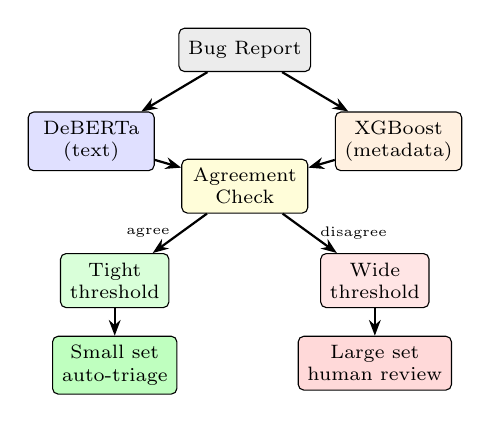
\begin{tikzpicture}[
  node distance=0.4cm and 0.5cm,
  box/.style={draw, rounded corners=2pt, minimum height=0.55cm,
              minimum width=1.6cm, font=\scriptsize, align=center},
  smallbox/.style={draw, rounded corners=2pt, minimum height=0.45cm,
              minimum width=1.3cm, font=\scriptsize, align=center},
  arr/.style={-{Stealth[length=2mm]}, thick},
  >=Stealth
]
% Input
\node[box, fill=gray!15] (input) {Bug Report};

% Two classifiers
\node[box, fill=blue!12, below left=0.5cm and 0.3cm of input] (deb) {DeBERTa\\(text)};
\node[box, fill=orange!12, below right=0.5cm and 0.3cm of input] (xgb) {XGBoost\\(metadata)};

% Agreement check
\node[box, fill=yellow!15, below=1.1cm of input] (agree) {Agreement\\Check};

% Two paths
\node[smallbox, fill=green!15, below left=0.5cm and 0.15cm of agree] (tight) {Tight\\threshold};
\node[smallbox, fill=red!10, below right=0.5cm and 0.15cm of agree] (wide) {Wide\\threshold};

% Outputs
\node[smallbox, fill=green!25, below=0.35cm of tight] (auto) {Small set\\auto-triage};
\node[smallbox, fill=red!15, below=0.35cm of wide] (review) {Large set\\human review};

% Arrows
\draw[arr] (input) -- (deb);
\draw[arr] (input) -- (xgb);
\draw[arr] (deb) -- (agree);
\draw[arr] (xgb) -- (agree);
\draw[arr] (agree) -- node[left, font=\tiny]{agree} (tight);
\draw[arr] (agree) -- node[right, font=\tiny]{disagree} (wide);
\draw[arr] (tight) -- (auto);
\draw[arr] (wide) -- (review);

\end{tikzpicture}
\caption{MACCP architecture. Two diverse classifiers produce independent predictions. Agreement routes bugs to a tight conformal threshold (small sets); disagreement routes to a wide threshold (large sets). Both partitions receive per-group coverage guarantees.}
\label{fig:architecture}
\end{figure}

\subsection{Base Classifiers}

\textbf{DeBERTa-v3-base}~\cite{he2021deberta} is a 184M-parameter transformer fine-tuned on bug report text (Summary~\texttt{[SEP]}~Description, truncated to 1500 characters). The disentangled attention mechanism processes contextual token embeddings through self-attention, and a classification head maps the pooled output to $K$ classes.

\textbf{XGBoost}~\cite{chen2016xgboost} processes TF-IDF features (500 dimensions from text) concatenated with engineered metadata: product encoding, creator bug count, severity, priority, operating system, platform, and component size computed from training data. We use 100 estimators with max depth 6.

These models are maximally architecturally diverse. DeBERTa learns contextual token representations through self-attention. XGBoost learns decision boundaries through gradient-boosted trees over numerical and categorical features. Their inductive biases are fundamentally different, making their agreement a strong reliability signal.

\subsection{MACCP Formulation}\label{sec:maccp-formulation}

Let $f_1$ (DeBERTa) produce a probability distribution $\mathbf{p}_1(x) = (p_1^{(1)}(x), \ldots, p_1^{(K)}(x))$ over $K$ classes, and let $f_2$ (XGBoost) produce top-1 prediction $\hat{y}_2(x)$.

\smallskip
\noindent\textbf{Step 1: Agreement indicator.}
\begin{equation}\label{eq:agreement}
A(x) = \indicator{\argmax_k\, p_1^{(k)}(x) \;=\; \hat{y}_2(x)}
\end{equation}

\smallskip
\noindent\textbf{Step 2: Partition the calibration set.}
Given $\calD_\text{cal} = \{(x_i, y_i)\}_{i=1}^{n}$:
\begin{align}
\calD_\text{agree} &= \{(x_i, y_i) \in \calD_\text{cal} : A(x_i) = 1\} \\
\calD_\text{disagree} &= \{(x_i, y_i) \in \calD_\text{cal} : A(x_i) = 0\}
\end{align}

\smallskip
\noindent\textbf{Step 3: Compute RAPS nonconformity scores} on $f_1$'s calibration softmax probabilities. Let $\pi_{(j)}(x)$ denote the $j$-th largest softmax probability and $k_i$ the rank of the true class $y_i$:
\begin{equation}\label{eq:raps-score}
s_i = \sum_{j=1}^{k_i} \Big(\pi_{(j)}(x_i) + \lambda \cdot \max(0,\, j - k_\text{reg})\Big)
\end{equation}
with $\lambda = 0.01$ and $k_\text{reg} = 5$.

\smallskip
\noindent\textbf{Step 4: Group-specific quantiles.}
For each group $g \in \{\text{agree}, \text{disagree}\}$:
\begin{equation}\label{eq:quantile}
\hat{q}_g = \Quantile\!\left(\frac{\lceil(|\calD_g|+1)(1-\alpha)\rceil}{|\calD_g|};\; \{s_i : i \in \calD_g\}\right)
\end{equation}

\smallskip
\noindent\textbf{Step 5: Prediction sets at test time.}
For a new instance $x$:
\begin{equation}\label{eq:pred-set}
\calC(x) = \left\{y : \sum_{j=1}^{\text{rank}(y)} \!\Big(\pi_{(j)}(x) + \lambda \cdot \max(0,\, j - k_\text{reg})\Big) \leq \hat{q}_{A(x)}\right\}
\end{equation}

\smallskip
\noindent\textbf{Coverage guarantee.}
From Mondrian CP theory~\cite{vovk2005algorithmic}:
\begin{equation}\label{eq:coverage}
\PP\!\big(Y \in \calC(X) \mid A(X) = a\big) \geq 1 - \alpha \quad \text{for each } a \in \{0, 1\}
\end{equation}

This is an instantiation of the Gibbs et al.~\cite{gibbs2025conditional} conditional coverage framework with a binary grouping function. The theoretical guarantee holds under exchangeability within each group.

\subsection{Explanation Layer}

A rule-based explanation generator attaches to each prediction: (i)~agreement status; (ii)~confidence tier (HIGH/MEDIUM/LOW); (iii)~reliability estimate citing historical accuracy of the partition; (iv)~top candidates from each model; and (v)~an action recommendation. Fig.~\ref{fig:explanation} shows examples for the agree and disagree paths.

\begin{figure}[t]
\begin{lstlisting}[style=explbox]
=== AGREE SINGLETON (AUTO-TRIAGE) ===
Prediction: {Platform}   | Coverage: 90%
Agreement:  AGREE (DeBERTa + XGBoost)
Confidence: HIGH (DeBERTa 0.91, XGBoost 0.88)
Accuracy:   ~90% for agree singletons
Action:     AUTO-TRIAGE

=== DISAGREE (NEEDS CAREFUL REVIEW) ===
Prediction: {UI, Core, Platform, SWT, Debug, ...}
Agreement:  DISAGREE
  DeBERTa -> UI (0.34)  |  XGBoost -> Core
Confidence: LOW
Action:     NEEDS CAREFUL REVIEW
\end{lstlisting}
\caption{Explanation examples. Agree singletons receive an auto-triage recommendation. Disagree predictions surface both models' candidates with an uncertainty flag.}
\label{fig:explanation}
\end{figure}

\subsection{Data Preparation and Temporal Split}

We use a strictly chronological split: 60\% train (oldest), 20\% calibration (middle), 20\% test (newest). Components are selected as the top-$K$ by training-set frequency. Components outside the top-$K$ are excluded, following Anvik~\cite{anvik2006should}: catch-all classes lack cohesive feature distributions and inflate nonconformity score variance during calibration, producing artificially wide prediction sets. Noise filtering removes INVALID, DUPLICATE, WONTFIX, and WORKSFORME resolutions, standard in Eclipse triage literature~\cite{lamkanfi2013eclipse,dipongkor2023transformer}. Canonical label mapping is computed from training data only and shared across both models.

The temporal split violates strict exchangeability between calibration and test data. Following Barber et al.~\cite{barber2023conformal} and Oliveira et al.~\cite{oliveira2024split}, we note that split conformal prediction maintains approximate validity under mild distribution shift, with coverage degradation proportional to the total variation distance between calibration and test distributions. We report empirical coverage at all $\alpha$ levels to verify this holds in practice.

% ============================================================
% IV. EXPERIMENTAL DESIGN
% ============================================================
\section{Experimental Design}\label{sec:design}

\subsection{Datasets}

Table~\ref{tab:datasets} summarizes the three datasets. Eclipse provides rich text and metadata for 30-component assignment. Mozilla Core targets 20 components with summary-only text. ServiceNow has no text fields, so only XGBoost + RAPS conformal is evaluated, demonstrating conformal prediction's applicability to non-textual SE triage data.

\begin{table}[t]
\caption{Dataset characteristics. All splits are strictly chronological.}
\label{tab:datasets}
\centering
\footnotesize
\setlength{\tabcolsep}{3pt}
\begin{tabular}{@{}lccccc@{}}
\toprule
\textbf{Dataset} & \textbf{Classes} & \textbf{Train} & \textbf{Cal} & \textbf{Test} & \textbf{Span} \\
\midrule
Eclipse     & 30 & 102{,}725 & 30{,}017 & 25{,}499 & 2001--2024 \\
Mozilla Core & 20 & 28{,}964 & 8{,}289 & 8{,}480 & 1998--2016 \\
ServiceNow  & 11 & 13{,}635 & 4{,}545 & 4{,}546 & 2016--2017 \\
\bottomrule
\end{tabular}
\end{table}

\textbf{Eclipse} (Zenodo 2024~\cite{lamkanfi2013eclipse}): 301K raw bugs reduced to 175K after noise filtering; top-30 components yield 158K bugs. Train period: 2001--2009, calibration: 2009--2014, test: 2014--2024.

\textbf{Mozilla Core} (BugsRepo~\cite{acharya2025bugsrepo,lamkanfi2013}): 45{,}733 resolved Core-product bugs from Mozilla Bugzilla with top-20 components (JavaScript Engine, Layout, DOM, Editor, XPCOM, etc.). Summary text only (no description field). Temporal split by bug ID: train 28{,}964 / cal 8{,}289 / test 8{,}480.

\textbf{ServiceNow} (UCI ML Repository): 22,726 IT incidents with 11 assignment group categories. No text fields available; only structured metadata (category, priority, impact, urgency). Train/cal/test split: 13,635 / 4,545 / 4,546.

\subsection{Baselines and Metrics}

\textbf{Baselines:}
(1)~DeBERTa RAPS---standard split conformal on DeBERTa alone;
(2)~XGBoost RAPS---standard split conformal on XGBoost alone;
(3)~MACCP (proposed)---Mondrian CP conditioned on agreement;
(4)~Softmax threshold baselines for selective prediction (non-conformal).

\textbf{Metrics:}
Empirical coverage (should be $\geq 1 - \alpha$);
mean and median prediction set size (smaller = more informative);
singleton rate (fraction of sets with exactly 1 class);
singleton accuracy (of singletons, fraction correct);
AUGRC (Area Under Generalized Risk-Coverage Curve~\cite{traub2024augrc}) with bootstrap 95\% CIs (10K resamples);
within-confidence-bin accuracy gaps (for RQ1).

\textbf{Alpha levels:} $\alpha \in \{0.01, 0.05, 0.10, 0.20\}$.

\textbf{Implementation:} DeBERTa fine-tuned using HuggingFace Transformers on 4$\times$ NVIDIA H100 GPUs. XGBoost via the xgboost library. Conformal prediction implemented directly (RAPS scores + quantile thresholds). Code available at \url{https://github.com/Git-Ansh/anomaly-detection-ci}.

% ============================================================
% V. RESULTS
% ============================================================
\section{Results}\label{sec:results}

\subsection{RQ1: Cross-Model Agreement Beyond Confidence}

Table~\ref{tab:agreement-gaps} presents within-confidence-bin accuracy for agree and disagree subsets on Eclipse. The agreement signal provides 43--69 percentage point accuracy gaps across all confidence levels.

\begin{table}[t]
\caption{Within-confidence-bin accuracy gaps (Eclipse, 30 classes). Agreement provides 43--69$\pp$ accuracy improvement independent of DeBERTa confidence.}
\label{tab:agreement-gaps}
\centering
\footnotesize
\setlength{\tabcolsep}{3.5pt}
\begin{tabular}{@{}lrccc@{}}
\toprule
\textbf{Confidence Bin} & $n$ & \textbf{Agree Acc.} & \textbf{Disagree Acc.} & \textbf{Gap} \\
\midrule
$[0.00, 0.30)$ & 1{,}341 & 78.0\% & 8.7\%  & +69.3$\pp$ \\
$[0.30, 0.50)$ & 3{,}910 & 77.0\% & 13.4\% & +63.6$\pp$ \\
$[0.50, 0.70)$ & 4{,}172 & 75.5\% & 19.6\% & +55.9$\pp$ \\
$[0.70, 0.85)$ & 3{,}594 & 79.3\% & 25.2\% & +54.2$\pp$ \\
$[0.85, 1.00)$ & 12{,}482 & 89.7\% & 46.6\% & +43.0$\pp$ \\
\bottomrule
\end{tabular}
\end{table}

\begin{figure}[t]
\centering
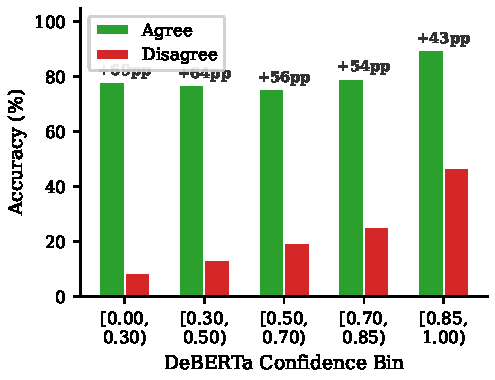
\includegraphics[width=\columnwidth]{figures/agreement_gaps.pdf}
\caption{Within-confidence-bin accuracy gaps (Eclipse). Even at the highest confidence ($\geq$0.85), XGBoost disagreement reduces accuracy by 43$\pp$.}
\label{fig:agreement-gaps}
\end{figure}

Even at the highest confidence level (0.85--1.0), where DeBERTa is most certain, XGBoost disagreement still reduces accuracy by 43.0 percentage points. This demonstrates that cross-model agreement captures reliability information entirely independent of softmax confidence, consistent with ensemble diversity theory~\cite{kuncheva2003measures,dietterich2000ensemble} but never previously quantified for conformal prediction conditioning.

Overall, the two models agree on 46.7\% of test bugs (11,913 / 25,499). When they agree, accuracy is 85.7\%; when they disagree, DeBERTa accuracy drops to 27.1\% while XGBoost retains 48.7\%. An oracle selecting the correct model when they disagree would achieve 80.4\%. Critically, 57\% of DeBERTa errors are caught by XGBoost, confirming genuine complementarity rather than correlated failure.

% -- Mozilla Core placeholder --
\smallskip\noindent\textit{Mozilla Core:} The pattern replicates. DeBERTa (39.1\%) and XGBoost (36.3\%) achieve comparable accuracy, with 26.8\% agreement rate. When they agree, accuracy is 75.8\%; when they disagree, 25.7\% (DeBERTa). Within-confidence-bin gaps range from 24.5 to 40.4$\pp$ in the four lowest bins, with an average of 29.0$\pp$. Only the highest confidence bin ([0.85, 1.0)) shows a weak 2.6$\pp$ gap, because DeBERTa is already 90.7\% accurate there regardless of agreement. These gaps are smaller than Eclipse's 43--69$\pp$ but still far exceed the 15$\pp$ threshold for practical significance, confirming that the agreement signal generalizes across bug tracking ecosystems.

\vspace{0.5em}
\noindent\fbox{\parbox{0.95\columnwidth}{\small\textbf{RQ1 Finding:} Cross-model agreement provides 43--69$\pp$ accuracy improvement within identical confidence bins, demonstrating that this signal is not redundant with single-model confidence. The binary agree/disagree indicator is a strong reliability signal for conformal prediction conditioning.}}

\subsection{RQ2: Prediction Set Efficiency}

Table~\ref{tab:rq2-alpha10} compares prediction set metrics at $\alpha = 0.10$ on Eclipse.

\begin{table}[t]
\caption{Prediction set comparison at $\alpha = 0.10$ (Eclipse, 30 classes). MACCP-agree achieves 61.2\% singletons with mean set size 2.30.}
\label{tab:rq2-alpha10}
\centering
\footnotesize
\setlength{\tabcolsep}{2.5pt}
\begin{tabular}{@{}lccccc@{}}
\toprule
\textbf{Method} & \textbf{Cov.} & \textbf{Mean} & \textbf{Med.} & \textbf{Sing.\%} & \textbf{Sing.Acc} \\
\midrule
DeBERTa RAPS       & 87.3\% & 5.30 & 5 & 23.5\% & 84.7\% \\
XGBoost RAPS        & 93.5\% & 3.12 & 3 & 20.1\% & 93.6\% \\
\midrule
MACCP overall       & 89.9\% & 5.61 & 6 & 28.7\% & 89.9\% \\
\quad agree (46.7\%)  & 91.5\% & \textbf{2.30} & \textbf{1} & \textbf{61.2\%} & 90.0\% \\
\quad disagree (53.3\%) & 88.4\% & 8.52 & 8 & 0.1\%  & ---    \\
\bottomrule
\end{tabular}
\end{table}

\begin{table}[t]
\caption{Prediction set comparison at $\alpha = 0.20$ (Eclipse, 30 classes).}
\label{tab:rq2-alpha20}
\centering
\footnotesize
\setlength{\tabcolsep}{2.5pt}
\begin{tabular}{@{}lccccc@{}}
\toprule
\textbf{Method} & \textbf{Cov.} & \textbf{Mean} & \textbf{Med.} & \textbf{Sing.\%} & \textbf{Sing.Acc} \\
\midrule
DeBERTa RAPS       & 79.0\% & 3.42 & 2 & 40.5\% & 77.9\% \\
XGBoost RAPS        & 87.3\% & 2.02 & 2 & 43.2\% & 87.8\% \\
\midrule
MACCP overall       & 81.4\% & 3.88 & 2 & 45.4\% & 83.8\% \\
\quad agree (46.7\%)  & 82.0\% & \textbf{1.56} & \textbf{1} & \textbf{76.2\%} & 85.3\% \\
\quad disagree (53.3\%) & 80.8\% & 5.92 & 5 & 18.3\% & 64.2\% \\
\bottomrule
\end{tabular}
\end{table}

\begin{figure}[t]
\centering
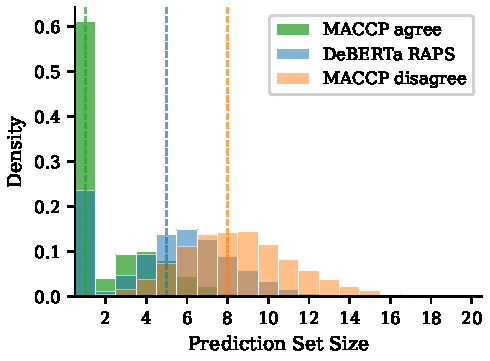
\includegraphics[width=\columnwidth]{figures/set_size_distribution.pdf}
\caption{Set size distributions at $\alpha = 0.10$ (Eclipse). The MACCP agree group concentrates at sizes 1--3 while disagree spreads across 5--15. DeBERTa RAPS peaks around 5.}
\label{fig:set-size}
\end{figure}

XGBoost RAPS achieves superior aggregate metrics (mean set size 3.12 vs.\ MACCP's 5.61). However, MACCP provides a capability that single-model RAPS cannot: an explicit, interpretable binary signal identifying which 47\% of predictions are reliable enough for automation (85.7\% accuracy) and which 53\% require human review. XGBoost RAPS produces uniformly tight sets but cannot distinguish reliable from unreliable predictions---the 6.4\% of singletons that are incorrect look identical to the 93.6\% that are correct. In operational triage systems, knowing \emph{which} predictions to trust is often more valuable than marginally smaller average set sizes.

AUGRC provides a threshold-free comparison: DeBERTa RAPS achieves 0.1644 [0.1611, 0.1676], XGBoost RAPS 0.1106, and MACCP 0.1384. The MACCP agree partition's operational value---61.2\% singletons at 90.0\% accuracy---is not captured by aggregate AUGRC, which treats all predictions equally.

The calibrated MACCP thresholds confirm the mechanism: $\hat{q}_\text{agree} = 0.953$ and $\hat{q}_\text{disagree} = 1.016$ at $\alpha = 0.10$. The tighter agree threshold forces smaller, more precise sets; the wider disagree threshold produces conservative sets ensuring coverage despite low base accuracy.

% -- Mozilla Core placeholder --
\smallskip\noindent\textit{Mozilla Core:} MACCP replicates. At $\alpha{=}0.10$, the agree partition (26.8\% of bugs) achieves mean set size 4.84 with 25.0\% singleton rate at 94.4\% singleton accuracy---compared to 0\% singletons for DeBERTa RAPS and 2.5\% for XGBoost RAPS at the same alpha. At $\alpha{=}0.20$, the agree partition achieves 45.8\% singletons at 93.2\% accuracy with mean set size 3.05, while DeBERTa RAPS produces only 18.3\% singletons. The effect is smaller than Eclipse (25\% vs 61\% singletons at $\alpha{=}0.10$) due to the lower base accuracy of both models (39\% and 36\% vs 54\% and 66\%), but the pattern is consistent: MACCP concentrates actionable predictions in the agree partition while correctly widening sets for uncertain cases.

% -- ServiceNow --
\smallskip\noindent\textbf{ServiceNow (XGBoost RAPS only).} With no text data available, only single-model conformal prediction is evaluated. XGBoost achieves 46.3\% test accuracy (majority baseline 24.5\%). Conformal results at $\alpha = 0.10$: 91.6\% coverage, mean set size 5.4, 14.1\% singleton rate, 96.2\% singleton accuracy. At $\alpha = 0.05$: 95.3\% coverage, mean set size 6.7, 7.2\% singletons, 98.2\% singleton accuracy. These results demonstrate that conformal prediction produces practically useful sets even with moderate base classifier accuracy and no text features.

\vspace{0.5em}
\noindent\fbox{\parbox{0.95\columnwidth}{\small\textbf{RQ2 Finding:} MACCP concentrates prediction efficiency where it matters most. The agree partition achieves 61.2\% singletons (vs.\ 23.5\% for DeBERTa RAPS) with mean set size 2.30. While XGBoost RAPS has better aggregate metrics, MACCP uniquely identifies \emph{which} predictions are automatable.}}

\subsection{RQ3: Coverage Under Temporal Shift}

Table~\ref{tab:coverage-all} reports empirical coverage across all alpha levels and datasets. Eclipse's test period (2014--2024) is 5--15 years after calibration (2009--2014), representing severe temporal shift: new components emerge, APIs evolve, and framework vocabularies change.

\begin{table}[t]
\caption{Empirical coverage across alpha levels. All datasets maintain coverage within 1--3$\pp$ of nominal despite temporal distribution shift.}
\label{tab:coverage-all}
\centering
\footnotesize
\setlength{\tabcolsep}{3pt}
\begin{tabular}{@{}lccccc@{}}
\toprule
$\alpha$ & \textbf{Nominal} & \textbf{Eclipse-30} & \textbf{Eclipse-31} & \textbf{Mozilla} & \textbf{ServiceNow} \\
\midrule
0.01 & 99\% & 97.0\% & 97.4\% & 96.9\% & 98.9\% \\
0.05 & 95\% & 92.6\% & 93.6\% & 92.0\% & 95.3\% \\
0.10 & 90\% & 87.3\% & 89.5\% & 87.7\% & 91.6\% \\
0.20 & 80\% & 79.0\% & 80.1\% & 79.7\% & 84.4\% \\
\bottomrule
\end{tabular}
\end{table}

\begin{figure}[t]
\centering
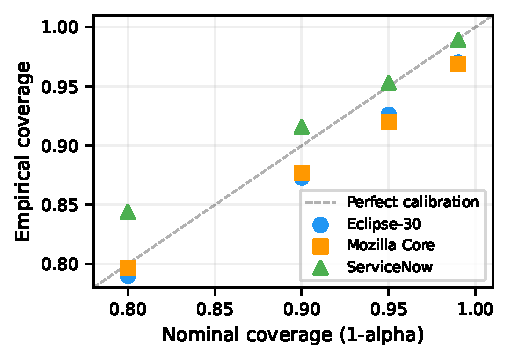
\includegraphics[width=\columnwidth]{figures/coverage_calibration.pdf}
\caption{Coverage calibration: empirical vs.\ nominal coverage. Points cluster near the diagonal, confirming approximate validity despite temporal shift.}
\label{fig:coverage-calibration}
\end{figure}

Across all datasets and alpha levels, empirical coverage is within 1--3 percentage points of nominal. We emphasize that this is an empirical observation, not a theoretical guarantee---the temporal split violates the exchangeability assumption required for Vovk's~\cite{vovk2005algorithmic} finite-sample coverage proof. Following Barber et al.~\cite{barber2023conformal}, we attribute the maintained coverage to the relatively mild total variation distance between calibration and test distributions, despite severe class proportion shifts.

The Eclipse-31 column includes the ``Other'' catch-all class, which grows from 2.2\% of calibration data to 27.2\% of test data. Even under this extreme shift, coverage at $\alpha = 0.10$ remains 89.5\%---only 0.5$\pp$ below nominal. The 30-class variant (excluding Other) shows slightly lower coverage (87.3\%), likely because the remaining classes have tighter probability mass, making the RAPS threshold more sensitive to distributional changes.

\vspace{0.5em}
\noindent\fbox{\parbox{0.95\columnwidth}{\small\textbf{RQ3 Finding:} Conformal coverage guarantees hold within 1--3$\pp$ of nominal across all datasets and alpha levels, despite temporal splits spanning 15--23 years. This is an empirical observation under conditions that violate strict exchangeability.}}

\subsection{RQ4: Cross-Dataset Generalization}

Table~\ref{tab:cross-dataset} summarizes results across all three datasets.

\begin{table}[t]
\caption{Cross-dataset summary. MACCP requires two competent models with diverse features; conformal prediction alone generalizes to metadata-only settings.}
\label{tab:cross-dataset}
\centering
\footnotesize
\setlength{\tabcolsep}{2.5pt}
\begin{tabular}{@{}lccccc@{}}
\toprule
\textbf{Dataset} & $K$ & \textbf{Best Acc.} & \textbf{MACCP?} & \textbf{Agree Sing.} & \textbf{Cov.?} \\
\midrule
Eclipse     & 30 & 66.0\% (XGB) & Yes & 61.2\% @ 90\% & Yes \\
Mozilla     & 20 & 39.1\% (DEB) & Yes & 25.0\% @ 94\% & Yes \\
ServiceNow  & 11 & 46.3\% (XGB) & No$^*$ & N/A & Yes \\
\bottomrule
\multicolumn{6}{@{}l}{\scriptsize $^*$No text model available; XGBoost RAPS conformal only.}
\end{tabular}
\end{table}

MACCP requires two competent base classifiers with architecturally diverse feature representations. On Eclipse (102K training samples with rich text and metadata), both models achieve sufficient accuracy for strong agreement signals (46.7\% agreement, 61.2\% singletons). On Mozilla Core (29K training samples, summary-only text), both models are weaker (39.1\% and 36.3\%) but MACCP still produces meaningful gains: 26.8\% agreement with 25.0\% singletons at 94.4\% accuracy in the agree partition. On ServiceNow, the absence of text fields precludes a second diverse model, so only single-model conformal prediction applies. Conformal prediction alone still provides valuable prediction sets: at $\alpha = 0.10$, ServiceNow achieves 91.6\% coverage with 14.1\% singletons at 96.2\% accuracy.

The explanation generator on Eclipse partitions 25,499 test bugs into operational categories: AUTO-TRIAGE 7,296 (28.6\%), AUTO-TRIAGE WITH CAUTION 20 (0.1\%), REVIEW SHORTLIST 2,525 (9.9\%), REVIEW NEEDED 1,367 (5.4\%), and NEEDS CAREFUL REVIEW 14,291 (56.0\%). The 28.6\% auto-triage rate with 90\% accuracy represents a substantial reduction in manual triage workload.

\vspace{0.5em}
\noindent\fbox{\parbox{0.95\columnwidth}{\small\textbf{RQ4 Finding:} Conformal prediction generalizes across all three SE triage ecosystems. MACCP replicates on both Eclipse (61.2\% singletons) and Mozilla Core (25.0\% singletons) with consistent agreement gaps. The effect scales with base model accuracy.}}

% ============================================================
% VI. DISCUSSION AND THREATS TO VALIDITY
% ============================================================
\section{Discussion and Threats to Validity}\label{sec:discussion}

\subsection{Practical Implications}

The MACCP framework partitions incoming bugs into three operational categories:

\begin{itemize}
\item \textbf{AUTO-TRIAGE (29\% of bugs):} Agree-group singletons. 90\% accuracy with formal coverage guarantee. Assign automatically with spot-check auditing.
\item \textbf{REVIEW SHORTLIST (10\% of bugs):} Agree-group non-singletons. Mean set size 2.30. Developer picks from 2--3 options.
\item \textbf{NEEDS CAREFUL REVIEW (56\% of bugs):} Disagree-group. Mean set size 8.52. Developer receives a shortlist with an uncertainty flag and both models' candidates.
\end{itemize}

The rule-based explanation layer provides interpretable context for the shortlist and careful-review categories, surfacing each model's top prediction and the historical accuracy of the partition. Even for the careful-review group, reducing 30 candidate components to a shortlist of ${\sim}$8 represents meaningful effort reduction.

\subsection{Connection to Related Work}

MACCP instantiates Mondrian CP~\cite{vovk2005algorithmic} within the Gibbs et al.~\cite{gibbs2025conditional} conditional coverage framework. The specific contribution is empirical: demonstrating that cross-model agreement is an exceptionally effective grouping variable for SE triage (43--69$\pp$ gaps). Compared to Kaur et al.'s~\cite{kaur2025trust} trust scores, our binary signal is simpler (no kNN computation, no hyperparameters) and maps directly to triage workflows. Compared to SACP~\cite{alami2025sacp} and CSA~\cite{ochoarivera2025csa}, we use less information from the auxiliary model (binary agreement vs.\ full score aggregation) in exchange for interpretability and practical simplicity. Future work could explore whether score aggregation methods yield further improvements.

\subsection{Why Metadata XGBoost Outperforms DeBERTa}

XGBoost achieves 66.0\% test accuracy versus DeBERTa's 54.5\% under the 15-year temporal split. Metadata features (product encoding, reporter history) are temporally invariant---a bug filed under ``Platform'' product carries the same signal in 2005 and 2020. Text vocabulary drifts substantially: API names, framework references, and coding paradigms evolve. This finding is consistent with Grinsztajn et al.~\cite{grinsztajn2022tree} showing tree-based models outperform deep learning on tabular data, and extends it to a temporal shift setting. The practical implication: in long-lived software projects, metadata-based models may be more reliable than text-based models for triage.

\subsection{Threats to Validity}

\textbf{Internal.}
(1)~The temporal split violates strict exchangeability. We concede this explicitly and report empirical coverage to verify approximate validity.
(2)~Label noise in Eclipse data: bugs may have been reassigned after initial triage; we use the final component as ground truth.
(3)~``Other'' class exclusion: we report both 30-class (excluding Other) and 31-class (including Other) results. Exclusion follows Anvik~\cite{anvik2006should} and is necessary for conformal calibration---catch-all classes lack cohesive feature distributions.

\textbf{External.}
(1)~MACCP requires two competent models with diverse feature representations. It fails when one model is too weak.
(2)~Eclipse and Mozilla Core are both Bugzilla-based open-source projects. Generalization to commercial bug trackers (Jira, Azure DevOps) with different taxonomies is untested.

\textbf{Construct.}
Singleton accuracy measures the automated component of the framework but does not capture developer effort savings for non-singleton predictions. A user study evaluating actual triage time reduction is needed.

% ============================================================
% VII. OPERATIONAL WORKFLOW
% ============================================================

Fig.~\ref{fig:workflow} shows how MACCP integrates into a development team's triage workflow.

\begin{figure}[t]
\centering
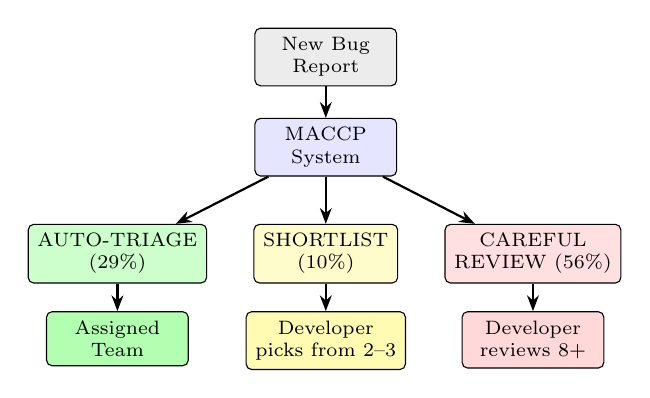
\begin{tikzpicture}[
  node distance=0.35cm and 0.4cm,
  box/.style={draw, rounded corners=2pt, minimum height=0.5cm,
              minimum width=1.8cm, font=\scriptsize, align=center},
  arr/.style={-{Stealth[length=2mm]}, thick},
]
% Input
\node[box, fill=gray!15] (bug) {New Bug\\Report};
\node[box, fill=blue!10, below=0.4cm of bug] (maccp) {MACCP\\System};

% Three outputs
\node[box, fill=green!20, below left=0.6cm and 0.6cm of maccp] (auto) {AUTO-TRIAGE\\(29\%)};
\node[box, fill=yellow!20, below=0.6cm of maccp] (short) {SHORTLIST\\(10\%)};
\node[box, fill=red!12, below right=0.6cm and 0.6cm of maccp] (review) {CAREFUL\\REVIEW (56\%)};

% Destinations
\node[box, fill=green!30, below=0.35cm of auto] (team) {Assigned\\Team};
\node[box, fill=yellow!30, below=0.35cm of short] (dev1) {Developer\\picks from 2--3};
\node[box, fill=red!15, below=0.35cm of review] (dev2) {Developer\\reviews 8+};

% Arrows
\draw[arr] (bug) -- (maccp);
\draw[arr] (maccp) -- (auto);
\draw[arr] (maccp) -- (short);
\draw[arr] (maccp) -- (review);
\draw[arr] (auto) -- (team);
\draw[arr] (short) -- (dev1);
\draw[arr] (review) -- (dev2);
\end{tikzpicture}
\caption{Operational workflow. MACCP routes bugs into three tiers: 29\% are auto-triaged (agree singletons at 90\% accuracy), 10\% receive a short shortlist, and 56\% are flagged for careful review with uncertainty context.}
\label{fig:workflow}
\end{figure}

% ============================================================
% VIII. CONCLUSION
% ============================================================
\section{Conclusion}\label{sec:conclusion}

We presented the first application of conformal prediction to multi-class software engineering triage, demonstrating that prediction sets with formal coverage guarantees are practically useful for 30-class bug component assignment. We showed that cross-model agreement between a DeBERTa transformer and an XGBoost tree ensemble provides 43--69 percentage point accuracy improvements within identical confidence bins---a reliability signal entirely independent of single-model confidence. We instantiated this finding as MACCP, a Mondrian conformal prediction framework conditioned on binary agreement, and demonstrated that the agree partition (47\% of bugs) achieves 61.2\% singleton prediction sets at 90\% accuracy with mean set size 2.30, enabling reliable automation of 29\% of all triage decisions. Conformal coverage guarantees hold within 1--3 percentage points of nominal levels across three datasets spanning 15--23 years of temporal shift.

\textbf{Limitations.} MACCP requires two competent classifiers with diverse feature representations. When one model is too weak, the agreement signal degrades. The temporal exchangeability violation means coverage guarantees are empirical, not theoretical, in our setting.

\textbf{Future work.}
(1)~Retrieval-augmented LLM explanations for the disagree group, surfacing similar historical bugs to help developers resolve ambiguous cases.
(2)~User study with developers measuring actual triage time reduction.
(3)~Extension to developer assignment (who should fix this?) rather than component assignment (which team?).
(4)~Online MACCP with adaptive conformal inference~\cite{gibbs2021adaptive} for continuous recalibration as component vocabularies evolve.
(5)~Investigation of score aggregation methods~\cite{alami2025sacp,ochoarivera2025csa} as alternatives to binary agreement partitioning.

% ============================================================
% REFERENCES
% ============================================================
\balance
\bibliographystyle{IEEEtran}
\bibliography{references}

\end{document}
